\documentclass[letterpaper,twocolumn,9pt]{article}
\usepackage{usenix,epsfig,endnotes,url,verbatim,array,fancyvrb,graphicx,grffile}

% For representing code in paragraphs.
\newcommand{\code}[1]{\texttt{#1}}


\begin{document}
\title{\Large \bf Web-based Data Analytics in Haskell}

%don't want date printed
\date{}
%make title bold and 14 pt font (Latex default is non-bold, 16 pt)

%for single author (just remove % characters)
\author{
{\rm Drew Haven, Eric Stratmann}\\
\{drew.haven, eric.stratmann\}@gmail.com
% copy the following lines to add more authors
% \and
% {\rm Name}\\
%Name Institution
} % end author

\maketitle


\begin{abstract}
Many people are interested in statistics, but providing an easy to use Website to analyze statistics can be difficult. We wanted to make it simple to create Websites to analyze arbitrary data, so we created a Haskell package that makes it easy to do this. We also wrote an example site using our package that analyzes data from the popular on-line game League of Legends. The Website allows users to lookup a variety of statistics and perform queries on the data.
\end{abstract}

\section{Introduction}

Analyzing statistics can be rewarding and insightful, but without an easy way to analyze new datasets doing so can be difficult. Statistics are useful in a verity of fields. For example, although no knowledge of statistics is required to play baseball, many fans of the sport love to analyze them. Since baseball is popular there are many Websites to analyze baseball data, but what about less popular data? Creating a site to analyze new sets of data can be time consuming.

Although the data being analyzed across different datasets may differ considerably, the sorts of queries that people are interested in are often similar. People would like to correlate different variables, filter on certain conditions, and retrieve subsets of the data. They would like to do calculations on the data (sums, averages, counts) and display this information in tables or charts. 

We have created FOOBAR~\cite{foobar}, a data analytics package written in Haskell that makes it convenient to write Websites to analyze arbitrary data. Our package allows developers to easily create a Website that allows users to query data from any dataset of their choosing and do other neat things. Since it is written in Haskell, our package takes advantage of Haskell features such as type safety. 

We created  a demo application using data from the on-line video game, League of Legends~\cite{lol}. League of Legends is a competitive Real Time Strategy games where teams of players compete against each other. The site allows users to view player information, analyze different variables, and other neat stuff. Users can analyze their own data to learn about their behavior in the game or look at more general data to see trends in game play. 

Todo: References don't work.
The rest of the paper is organized as follows. Section \ref{background} provides some background. We discuss our package in section \ref{package}. Section \ref{site} looks at our example site. In section \ref{future} we discuss possible future directions of our work. We provide an analysis of our results in section \ref{analysis}. Finally, section \ref{conflusion} concludes.

\section{Background, Technologies Used, Related Work, etc.}
\label{sec:background}

\subsection{Yesod}

Yesod~\cite{yesod} is one of several Web frameworks written in Haskell. Features of Yesod include templates, a persistence model, etc. Writing a Website in a Haskell framework allows developers to take advantage of Haskell features, such as type safety, which helps them write secure sites.

Yesod uses both MVC and REST. MVC is a paradigm for writing Websites that separates data and data logic (model) from the presentation of the data (view). REST is a convention for URLs so that sites can have a consistent pattern for accessing resources. 

To write controllers, developers can use Yesod's monads, Handler and Widget. These build up HTML, CSS, and Javascript, and allow modifying and reading HTTP headers. These monads are instance of MonadIO which allows controller pages to execute arbitrary IO actions as well as generating the page. See Figure \ref{controller} for an example controller 

Like most other frameworks, Yesod provides templates to make writing HTML, CSS, and Javascript easier. The templates provide basic variable substition and and control statements, as well as support for simplified stuff. See Figure \ref{hamlet} for an example of Hamlet, Yesod's HTML tempalting system, which is used in the controller in Figure \ref{controller}.

Yesod uses Haskell's types to provide functionality that often are impossible in other languages. Type safety prevents many security vulnerabilities by ensuring that malicious code isn't used. Type inference allows more concise code by automatically detecting what model the developer is querying.


\begin{figure}[]
\begin{verbatim}
getGameIndexR :: Handler RepHtml
getGameIndexR = do
  (games, opts) <- paginateSelectList 10 [] []
  defaultLayout $ do
    let list = $(widgetFile "game/list")
    setTitle "Game Index"
    toWidget [cassius|
      ##header {
        float: left;
        color = #{color}}
    |] 
    $(widgetFile "game/index")
\end{verbatim}
    \caption{Sample Yesod Controller}
    \label{controller}
\end{figure}

\begin{figure}[]
\begin{verbatim}
^{pager opts}

<table.game-list>
<thead>
  <tr>
    <th>
      Teams
    <th>
      Queue
    <th>
      Date Added
<tbody>
  $forall game <- games
    <tr data-href=@{GameViewR (fst game)}>
      <td.champs>
        ^{portraits champions (snd game)}
      <td.queueType>
        #{gsqueueType (gameGameStats (snd game))}
      <td.created>
        #{gameFormattedCreateTime (snd game)}
\end{verbatim}
    \caption{Sample Hamlet File}
    \label{hamlet}
\end{figure}

\subsection{Persistent}

Persistent is a library developed for Yesod to facilitate data access.  It attempts to make data access type safe, concise, declarative and independent of the underlying data store.  It uses a mixture of type-classes to achieve this, as well as various language extensions to make some of tricks possible.  The three major pieces of the puzzle are the type classes \code{Persistback-end b m}, \code{PersistField val}, and \code{PersistEntity val}.

The core of Persistent is the \code{Persistback-end b m} typeclass, which defines the basic operations on the database such as \code{insert}, \code{update}, \code{delete}, and \code{get}.  An interesting point is it encodes the back-end type in the \code{b} parameter, but also specifies the constraints \code{Monad m}, \code{Monad (b m)}, \code{MonadIO m} and \code{MonadIO (b m)}.  This forces the back-end type to provide the mechanism for accessing IO to get to interface with the database without making any specific statements about how or where \code{Persistback-end} instances can be used, as they all return values in the \code{b m} monad.

Persistent deals with types by having a restricted set of types that it uses to interface with the database, the \code{PersistValue} type.  These types closely resemble JSON or BSON types, as it includes a few primatives, null, and the two collection types \code{PersistList [PersistValue]} and \code{PersistMap [(Text, PersistValue)]}.  The library ensures that the back-end can store values of these types to limit dependencies and coupling between the application data types and the database's internal representation.

Any datatype that can be stored as a database column needs to be an instance of the \code{PersistField} typeclass.  This typeclass handles the marshalling to and from \code{PersistValue}s.  The close resemblance of \code{PersistValue} to JSON types, specifically \code{Data.Aeson.Value}, allowed us to write code to do an instance of \code{PersistField} for \code{Data.Aeson.Value}, and from that we could utilize the same \code{FromJSON} and \code{ToJSON} instances we wrote from the parsing code to implement a \code{PersistField GameType} instance that we could use to store the game statistics data in the database.  The library understands how to represent \code{PersistValue}s in MongoDB in a way that preserves their structure, which gave us the ability to do deep inspection of the data in the database, which was essential for our query filters and map reduce code.

The final piece of the puzzle is the \code{PersistEntity val} typeclass, which is the one we worked with the most.  This typeclass defines the code for converting a top-level data type to or from column data, the columns present on the data type and unique key constraints.  The interesting piece are the columns, which are defined through the \code{EntityField} data type, which is a type family parameterized by the type of \code{val}.  \code{TypeFamilies} is an extension I haven't seen used often, but is used well in this context.  In this case it is used to allow different constructors of the datatype to take on different types.  This is one of the more interesting examples of how Yesod uses typeclasses to ensure type safey.  See Figure \ref{EntityField} for an example definition.

\begin{figure}[]
\begin{verbatim}
data EntityField (GameGeneric backend) typ
    = typ ~ (Key backend (GameGeneric backend)) => GameId 
    | typ ~ UTCTime   => GameCreated
    | typ ~ Bool      => GameRanked
    | typ ~ Int       => GameGameId
    | typ ~ Int       => GameLength
    | typ ~ GameStats => GameGameStats
    | typ ~ Text      => GameTeamPlayerSummoner Text
    | typ ~ Text      => GameOtherTeamPlayerSummoner Text
\end{verbatim}
    \caption{EntityField declarations for GameGeneric backend}
    \label{EntityField}
\end{figure}

When put together these components create a very declarative way to define data and queries.  Much of the definition can be done through Template Haskell functions, such as \code{derivePersistField} or \code{mkPersist}.  These will define the datatypes and their instances for the most common case.  For our case we wanted to define query columns that inspect the data more deeply than the first layer.  To do that we had write our own \code{PersistEntity} definitions.  It was surprisingly easy to add additional columns, however the details of how Persistent builds queries restricted them to only be simple column comparisons in MongoDB, multi-column functions may be possible in SQL.

Filters are created through comparison functions, which are analogs for familiar comparison functions, such as less-than, equals and set membership.  They are defined by the \code{PersistFilter} data type, and Yesod provides more convenient creation functions.  The Filters also encode type-safety of the comparison (Figure \ref{Filter}).  Note the Rank2Type for \code{typ} which enforces a match between the value and the field's type.  Also note that \code{v} represents the model type, which ensures all filters correspond to columns on the same data type.
\begin{figure}[]
\begin{verbatim}
    data Filter v = forall typ . PersistField typ => 
        Filter { filterField :: EntityField v typ
               , filterValue :: Either typ [typ]
               , filterFilter :: PersistFilter
               }
        | FilterAnd [Filter v]
        | FilterOr [Filter v]
\end{verbatim}
    \caption{EntityField declarations for GameGeneric backend}
    \label{Filter}
\end{figure}
Select queries naturally follow from their filters, which encode almost all information needed to make the query.  The select only requires a few additional options such as limits and offsets before it can be executed.

Persistent is a very elegant system for database access, and was a pleasure to work with on this project.  It does make a few assumptions about your data to enable its optimizations.  Examples include an inability to model relational data and a restricted set of operations.  Current work on Persistent is attempting to address this by splitting the backend from the query interface so more complex queries can be executed on backends that support them.

\subsection{MongoDB}

Our backend used MongoDB~\cite{mongo}, a documented-oriented database. MongoDB stores data in BSON, a binary-encoded serialization of JSON-like documents, with a few extenstions for additional data types.  The MongoDB query system includes a simple query system that allows for simple operations analogous to non-relational SQL statements.  This is how all basic CRUD operations are performed.  It also has a second query system that utilizes map-reduce.  The map-reduce system uses JavaScript functions to run queries across documents and shared databases.  MongoDB is schemaless in that the documents have no defined structure or types.  This creates a burden on the client to ensure data is consistent and well-formed.

\subsection{Flot}

To generate charts, we use Flot~\cite{flot}, a JavaScript charting library. We originally used the Chart package, but switched to Flot for compatibility reasons and because JavaScript charts are more dynamic. Since Flot did not have Haskell bindings, we had to write our own. 

\subsection{League of Legends}

League of Legends~\cite{lol} in an on-line Real Time Strategy game. Although the details are not important since we have chosen any other dataset to analyze, we provide a quick introduction of the important concepts to put the examples into context. Players (also known as summoners) fight in teams of five against each other using characters known as Champions. The object of the game is to advance to and destroy the other side's base. Players can advance towards this objective by killing other players and completing secondary objectives which they use to gain additional power and gold which is used to purchase upgrades. People are interested in different statistics of summoners and champions, such as their kill and death rates, total gold gained and towers destroyed.

Particularly interesting statistics could arise from comparisons, such as win-rate compared to game length, or across many players you could look at the number of secondary objectives completed compared to the average match-making rating of the team.

\section{Description of our project}
\label{package}

\subsection{Data backend}

\begin{figure*}[t]
\begin{verbatim}
type Game = GameGeneric backend
type GameId = Key backend Game
GameCreated :: EntityField Game UTCTime
GameGameStats :: EntityField Game GameStats

selectList :: (PersistEntity val, PersistBackend b m) => [Filter val] ->
              [SelectOpt val] -> b m [(Key b val, val)]
selectList [GameCreated <. time] [LimitTo 10] :: PersistBackend b m => b m [(GameId, Game)]
\end{verbatim}
    \caption{Query stuff}
    \label{querycode}
\end{figure*}

Data is represented by a small collection of data types, the major ones being \code{GameStats} and \code{PlayerStats}.  In short, a game is represented by \code{GameStats} which has a field for each team which contains a map from player name so to \code{PlayerStats}, which in turn contains a \code{Map Text Int} which contain the various statistics for the player.  Data is stored in MongoDB and represented fairly close to the original data format.  This is conveniently achieved by using the \code{FromJSON} and \code{ToJSON} instances defined for the original parser.  As the project progressed we altered the data format by performing some transformations on the raw data to remove unnecessary layers of data types and provide more convenient indexing, this required that the data parsing for raw data and database data diverged.  We wrote a simple instance for \code{PersistField} for \code{Data.Aeson.Value} and some TemplateHaskell functions to generate the instances for us.  Basic queries use this interface.

A large part of our Yesod code was written for our map-reduce query interface.  The interface is modeled on Persistent, and is designed to be an alternate query interface.  One major difference is that we want the map-reduce queries to return semi-arbitrary data with respect to the underlying data model, so we cannot return a clear type.  For example, one column that might be requested could be an average of many \code{Int} columns which is represented as a \code{Float}.  Queries also need to be dynamically definable so that users can specify what data they want to access.  We compromised by returning the opaque \code{Value} type, which corresponds to BSON values, and provided a casting operation to safely coerce the value to the correct type.  This puts a burden on the programmer to keep track of which columns are which, but it was deemed acceptable for the prototype.

The query API essentially comes down to two pieces.  The main \code{mapReduce} (Figure \ref{mrapi}) function which is similar to the \code{selectList} function of Persistent.  The other piece is the \code{Queryable} type-class (Figure \ref{queryable}) which defines the functions for transforming columns into filters and map-reduce code.  The goal is to make it easy to define new columns on whatever your data type might be.  To achieve this, most of the functions in \code{Queryable} have default implementations and there are a suite of helper functions which work with the default implementations to limit how much needs to be defined for each column, for example \code{simpleMap} takes a selector and produces the proper code to be inserted into the default map function to extract that item.  There is also an implicit \code{\_count} column which stores the number of documents contributing to the data.

\begin{figure*}[t]
\begin{verbatim}
mapReduce :: (PersistBackend Action m, Applicative m, Queryable model)
  => QueryColumn model typ                 -- ^ The column to use a key.
  -> [QueryFilter model]                   -- ^ A list of filters.
  -> forall typ0. [QueryColumn model typ0] -- ^ A list of columns to select for the output.
  -> Action m [(Label, M.Map Label Value)]
\end{verbatim}
    \caption{Map-Reduce API}
    \label{mrapi}
\end{figure*}

\begin{figure*}[t]
\begin{verbatim}
class PersistEntity model => Queryable model where
    -- Column definitions
    data QueryColumn model :: * -> *
    queryColumnName     :: QueryColumn model typ -> UString
    queryFilter         :: QueryColumn model typ -> Value -> Document
    queryKeyCode        :: QueryColumn model typ -> Javascript
    queryMapCode        :: QueryColumn model typ -> Javascript
    queryReduceCode     :: QueryColumn model typ -> Javascript
    queryFinalizeCode   :: QueryColumn model typ -> Javascript
    queryCastResult     :: (Val typ) => QueryColumn model typ -> Value -> Maybe typ
    queryMapFunc        :: QueryColumn model typ -> forall typ0. [QueryColumn model typ0] -> Javascript
    queryReduceFunc     :: forall typ0. [QueryColumn model typ0] -> Javascript
    queryFinalizeFunc   :: forall typ0. [QueryColumn model typ0] -> Javascript
    queryCollection     :: QueryColumn model typ -> UString
\end{verbatim}
    \caption{Map-Reduce API}
    \label{queryable}
\end{figure*}

The JavaScript can be essentially arbitrary.  We created a default form which we focused on while providing the ability to define arbitrary code.  This did limit what we were able to do with the system, but our goal was to create a working product and not to perfect the interface.  Our default form was to define a method for selecting a value, which could be used as either a key or a value.  The map step extracts the key with \code{queryKeyCode}, then for each column it runs \code{queryMapCode} which adds the value to the result object which is then emitted with the key.  The reduce code merges two records by iterating over every column and using the corresponding code which can be defined through \code{simpleReduce} by providing just an operator.  The finalize step is run after all the reductions have been performed, and also iterates over all the columns; there are simple helper functions for either totals or averages.

The advantages of this interface are that control of the columns is in the hands of the programmer and can theoretically be anything the user could write directly, however once written they can be composed, combined, and reused easily.  The queries are also very declarative and type-safe, preventing the programmer from mixing columns for different models or providing the wrong type to a filter.

There are three major drawbacks.  The first is that the user has to directly specify JavaScript which is error prone and breaks the abstraction provided by Persistent; the helper functions alleviated some of this, but even for our simple queries we were unable to avoid writing JavaScript expressions.  There may be a way around this, but we were unable to find one that could be implemented on our timescale.  The second drawback is that each new column may require defining a pattern-match on many functions.  This depends on how complex the JavaScript is and can be fixed by defining some additional functions to reduce repetition.  The final drawback is that the results are returned as BSON \code{Value}s; requiring the programmer to cast the value to a \code{Maybe typ} through \code{getResultValue :: (Val typ, Queryable model) => QueryColumn model typ -> M.Map Label Value -> Maybe typ}.

\subsection{Chart generation}

Our Website displays appropriate information using Javascript charts. While some data is best presented in tabular form, charts can visually display the relationship of different variables in a way that is easy for people to understand. In particular, we thought viewing a chart would help users view correlations between two different variables. Figure \ref{chart} shows a sample chart.

We used the Flot Javascript charting package. Flot charts are generated using Javascript and displayed on an HTML Canvas element. While we had originally tried generating static chrats, that did not give us the same level of functionality as the Javascript charts. Although we didn't end up using any of this functionality, it would have allowed users to sort charts in the browser, click on different elements to go to the appropriate page, etc. 

While it is possible for developers to manually generate Javascript to create Flot charts, we created a Haskell API that allows developers to specify their charts in Haskell. The API takes a list of display parameters (such as titles, chart size, orientation, etc.) and a list of data points in the form \code{[(key, value)]} .The chart automatically takes care of including any necessary HTML, Javascript, and CSS and can simply be included anywhere in the page. Figure \ref{chartcode} shows a page that uses the chart API. \code{myChart} sets a few chart options and the data is queried from the database. 

\begin{figure}[]
\begin{verbatim}
getFooR :: Handler RepHtml
getFooR = do
    data <- runDB blah buildQuery blah
        (QuerySomething foo) []
        [Query Something])
    let chart = makeChart myChart data
    ...

myChart :: Widget
myChart = 
    setTitles "XAxis" "YAxis" "Title" $
    setHorizontal True $
    setSize 600 400 $
    barChart
\end{verbatim}
    \caption{Chart API}
    \label{chartcode}
\end{figure}

\begin{figure}[h]
    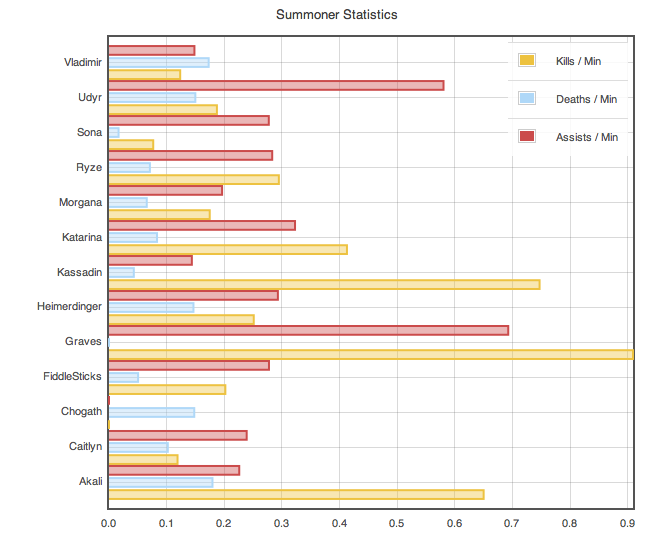
\includegraphics[width=80mm]{imgs/chart.png}
    \caption{Chart}
    \label{chart}
\end{figure}

\subsection{League of Legends Logs}

\begin{figure}[]
\begin{verbatim}
11/2/2011 00:25:47.609 [DEBUG] com.riotgames.platform.gameclient.domain.PlayerParticipantStatsSummary ENDOFGAME: Player: null has items: ,1042
11/2/2011 00:25:48.218 [DEBUG] com.riotgames.platform.gameclient.module.services.RemoteObjectGenerator Got async message: (mx.messaging.messages::AsyncMessageExt)#0
  body = (com.riotgames.platform.gameclient.domain::EndOfGameStats)#1
    basePoints = 69
    completionBonusPoints = 0
    difficulty = (null)
    elo = 0
    eloChange = 0
    experienceEarned = 0
    gameId = 245368572
    gameLength = 1839
    gameMode = "CLASSIC"
    gameType = "MATCHED_GAME"
    newSpells = (mx.collections::ArrayCollection)#2
      filterFunction = (null)
      length = 0
      list = (mx.collections::ArrayList)#3
        length = 0
        source = (Array)#4
        uid = "640DA889-2833-A482-F73E-632B62D95119"
      sort = (null)
      source = (Array)#4
\end{verbatim}
    \caption{Sample League of Legends Log}
    \label{samplelog}
\end{figure}

\begin{figure}[]
\begin{verbatim}
type Object      = M.Map T.Text ASValue

data ASValue = ASNumber N.Number
             | ASString T.Text
             | ASBoolean !Bool
             | ASNull
             | ASDate T.Text
             | ASArray !Integer (V.Vector ASValue)
             | ASObject T.Text !Integer Object
             deriving (Show, Eq)
\end{verbatim}
    \caption{ActionScript object descriptions}
    \label{asvalue}
\end{figure}

The League of Legends client is written in Adobe Air and runs in the background while games are in progress. Data from the League of Legends game client is dumped to log files.  It has a standardized format, but the most interesting data for our case are the end-of-game stats, which are dumped out by an object dumping routine.  Data types in these dumps are fairly straight-forward and can be mapped onto JSON data types, but to do so requires parsing the structure of the dump, which is based on indentation.

The first phase of our parsing is to parse object dumps into an \code{ASValue} datatype, which is modeled after \code{Data.Aeson.Value} and described in figure \ref{asvalue}.  The parsing code is written with Attoparsec, and is straightforward other than the indentation.

Indentation is tracked by wrapping the \code{Parse} monad in a reader transformer that stores the number of spaces on the current indentation.  Every key-value pair of an object or entry in an array first checks for the corresponding level of indentation.  When a new object or array is encountered, the indentation is incremented for the recursive call, and if the indentation fails to parse it simply signifies the end of the object and the \code{many} combinator will return the results parsed so far.

Once the end-of-game log messages have been extracted and the data parsed into \code{ASValue} it can be converted one-to-one into \code{Data.Aeson.Value} through an appropriate \code{ToJSON} instance.

Since we want to represent the data internally in a form different from that of the logs---note the awkward \code{ArrayCollection} and \code{ArrayList} objects in the sample that are essentially just a list or vector---we needed to write two functions to parse the JSON.  For the database store we used the TemplateHaskell derivied \code{FromJSON} and \code{ToJSON} instances.  For parsing the raw data we hand-wrote a more complicated parser that does a few minor data transformations along the way, such as indexing some arrays by a key and removing some unnecessary layers of data and duplicate fields.

In the end we can convert logs into \code{ASValue}; \code{ASValue}s to and from \code{Data.Aeson.Value}s; and \code{Data.Aeson.Value}s to and from \code{GameStats}.  In our implementation, the uploader client does the conversion from logs to JSON, which is then serialized and uploaded to the server which treats it as the raw JSON form and parses it into \code{GameStats} which it wraps in a \code{Game} model and stores in the database.

\subsection{League of Legends Log-Upload Client}

The first implementation of the uploader used the parsing code mentioned above and \code{Network.HTTP} to upload the resultant JSON to a server.  This portion of the code is fairly straight-forward Haskell.  However, this required the user to run the command from a terminal and provide the directory of the logs as an argument to the program, which is outside the comfort zone of many potential users.

The first revision involved querying the windows registry through the \code{System.Win32} library.  This proved useful, creating a binary that could be simply double-clicked to perform the uploading, though the output was still displayed in a console.  When distributing the program to alpha testers we found that the registry keys used were not consistent across systems.  This was solved by querying multiple keys until one yielded a result, but even that was insufficient as some users were running the program without having run the installer process and so had no registry keys, and at least one of our alpha testers was also using a non-default directory.

The solution is to prompt the user for the location of the program which forces us to move towards a GUI.  Some brief research suggested wxWidgets as a good cross-platform GUI system.  We set up a system which built a GUI and ran the UI in one thread after doing a directory look up and prompting the user if necessary, then spawned a worker thread to do the parsing and uploading.  The worker thread appended its log messages to a \code{Control.Concurrent.STM.TVar}, which is polled by the GUI to update its display and give the user easier access to error messages and progress information.  We used a \code{ReaderT} wrapper around IO to run actions in a way that they would have access to the log.

The program compiled, but we had difficulty distributing it due to DLL dependencies.  GHC statically links most libraries by default, which was desired for distribution, however when compiling the wx code, it attempts to link many things dynamically including \code{libstdc++}.  Even locating the libraries and placing them in path, other libraries such as \code{libgcc\_s\_dw2-1} were requested by the binary, but weren't present in the Haskell Platform, wxPack (the wxWidgets distribution), or MinGW (providing gcc).  After going through a few hours of tracking down DLLs, adding static compilation flags, and recompiling, we abandoned the GUI for windows users due to time constraints. 

At this time I believe a better approach to a cross platform GUI would be to use another language such as Java which has a track-record of creating cross-platform GUIs. Other GUI libraries for Haskell such as GTK are worth a look to determine if they suffer the same problems as wxWidgets.

\section{League of Legends Site}
\label{site}

To test our data analytics package, we wrote a Website to display League of Legends statistics. Although the Website is fairly simple for an analysis Website, building the site helped us in developing our query interface. The Website allows users to upload games, view information about games, viwe champion data, and perform analyzis on summoner data.

Our summoner page, seen in \ref{todo}, displays aggregate information about a summoner across all uploaded games the summoner played in. The data is viewable in both table and chart format, and the columns are customizable about the user.

Our backend is capable of performing more powerful queries, but we did not have enough time to code more pages to display this functionality. Ideally, users would be able to specify arbitrary queries, giving custom filters, keys, etc. 

In Figure \ref{list}, we can see a list of games. Probably want a more interesting picture though.

\begin{figure}[h]
    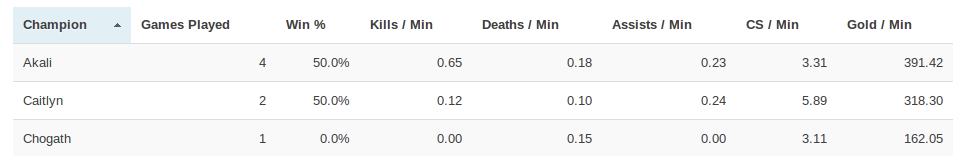
\includegraphics[width=80mm]{imgs/stats.png}
    \caption{Statistics for a summoner}
    \label{chart}
\end{figure}

\begin{figure}[h]
    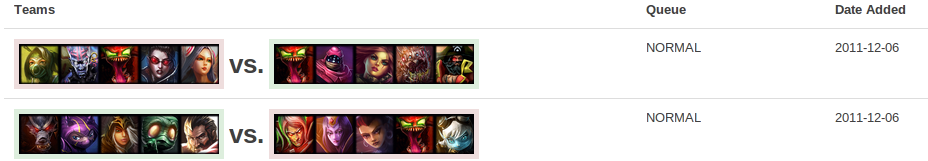
\includegraphics[width=80mm]{imgs/gamelist.png}
    \caption{Game list}
    \label{list}
\end{figure}

\section{Future Work}
\label{future}

Although we are happy with the progress we made on our project, neither the backend nor the Website are production quality. To bring our project to that level, we would need to make a few changes. 

* Static file handling.  Yesod is not optimized for it.

Our website does not include user accounts. Although user accounts are not neccessary to simply analyze existing data, we need some sort of permissions to disallow the unauthorized modification of data.

Development branch of Persistent has abstracted the query interface, making this work easier.

We had mixed feelings about working with Yesod. Although the framework takes advantage of serveral Haskell features, the framework is not as mature as those available for other languages. For example, there was little documentation except for the most basic features. This is not too surprising since Yesod is less than two years old and has only a few core developers. 

\section{Analysis}
\label{analysis}

We learned X.

Features X, Y, and Z of Haskell/Yesod/etc. were lacking and we'd like to see some improvements.

Features X, Y, and Z of Haskell/Yesod/etc. were great and gave us the following benefits.

Overall we were pleased/displeased/had no strong feelings about our project.

\section{Conclusion}
\label{conclusion}

Data analytics can be fun and exciting. We created a Website to analyze League of Legends data, but can be used with a variety of data.

Our project shows that Haskell is a good/ok/bad language for data analytics, although X. 

{\footnotesize \bibliographystyle{acm}
\bibliography{paper.bib}}

\end{document}
